\documentclass[tikz,border=2pt]{standalone}
\usepackage{amsmath,amssymb}
\usepackage{tikz}
\usetikzlibrary{arrows.meta}

\begin{document}
% A directed network: each edge has an orientation; A -> B allows travel from A to B only.
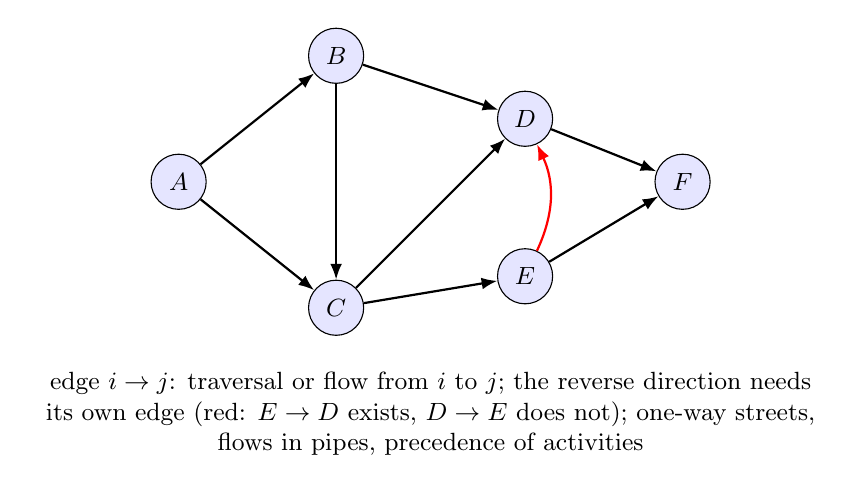
\begin{tikzpicture}[every node/.style={font=\small}, >={Latex[length=2mm]}, v/.style={draw, circle, fill=blue!10, minimum size=7mm, inner sep=0pt}]
	\node[v] (A) at (0,0) {$A$};
	\node[v] (B) at (2,1.6) {$B$};
	\node[v] (C) at (2,-1.6) {$C$};
	\node[v] (D) at (4.4,0.8) {$D$};
	\node[v] (E) at (4.4,-1.2) {$E$};
	\node[v] (F) at (6.4,0) {$F$};
	\draw[->, thick] (A) -- (B);
	\draw[->, thick] (A) -- (C);
	\draw[->, thick] (B) -- (C);
	\draw[->, thick] (B) -- (D);
	\draw[->, thick] (C) -- (D);
	\draw[->, thick] (C) -- (E);
	\draw[->, thick] (D) -- (F);
	\draw[->, thick] (E) -- (F);
	\draw[->, thick, red] (E) to[bend right=25] (D);
	\node[anchor=north, align=flush center, text width=10cm] at (3.2,-2.3) {edge $i\to j$: traversal or flow from $i$ to $j$; the reverse direction needs its own edge (red: $E\to D$ exists, $D\to E$ does not); one-way streets, flows in pipes, precedence of activities};
\end{tikzpicture}
\end{document}
